\documentclass{amsart}
\title{Attack on Galois RLWE}
\author{Kristin Lauter, Kate Stange, Hao Chen}

\usepackage{macros}
\usepackage{float}
\usepackage{url}
\usepackage{placeins}
\usepackage{hyperref}

\usepackage{algpseudocode}
%\usepackage{algorithmic}
\usepackage{algorithm}
\usepackage{physics}

\begin{document}
\maketitle

\begin{abstract}
We describe a new attack on the Ring learning-with-errors (RLWE) problem based on chi-square test, and give examples of Galois number fields vulnerable to our attack. We also analyze the security of cyclotomic extensions under our attack using Fourier analysis on finite fields.

%Also, we sharpen the attack in [ELOS] and give examples of vulnerable instnaces of cryptographic size. Finally, we discuss the effect of modulus switching on our attacks.
\end{abstract}

\section{Introduction}
The Ring learning with errors (RLWE) problem, proposed in [LPR], is a variant of the traditional learning with error (LWE) problem, and is an active research area in lattice based cryptography. The hardness result of [LPR] reduces certain Gap-SVP problems to an RLWE problem for 2-power cyclotomic fields. The contribution of [EHL] paper, [ELOS]
The [Toolkit] paper describe an efficient algorithm to generate samples from the dual version of RLWE for general cyclotomic fields, and the [DD] paper discusses efficient ways of sampling from the non-dual version. In our paper, we restrict ourselves to the non-dual variant of RLWE.

\subsection{Contributions}

\subsection{Techniques}

\subsection{Organization}

In section \ref{sec: background}, we recall the canonical embedding of number fields and the central definitions related to RLWE.

In section \ref{sec: s-to-d}, we review prime factorizations in Galois extensions and prove a search-to-decision reduction for Galois extensions $K$ and unramified primes of any degree.

In section \ref{sec: chi-square}, we introduce an attack to RLWE problems based on the chi-square statistical test. The time complexity of our attack is $O(\frac{n}{f}q^{2f})$ for the decision version RLWE and for an intermediate problem which we denote by $\SRLWE(\cR,\fq) (see \ref{def: })$.

In section, \ref{sec: sub-cyclotomics}, we give examples of subfields of cyclotomic field which are vunlerable to our attack outlined in section \ref{sec: chi-square}, where the moduli $q$ has residue degree two. We then try to explain why degree two moduli are more likely to be vulnerable than degree one primes, i.e., primes that splits completely in the number field $K$.

In section \ref{sec: }, under some simplifying assumptions, we show that general cyclotomic extensions, with an unramified prime as the modulus $q$, are invulnerable to our attack. Our argument uses Fourier analysis on finite fields in an essential way.

In section, \ref{sec: ramified-prime}, we show that the attack in [ELOS] applies to prime cyclotomic fields, if the moduli is divisible by the unique ramified prime.



\section{Background} \label{sec: background}

Let $K$ be a number field of degree $n$ with ring of integers $R = \cO_K$ and let $\sigma_1, \cdots, \sigma_n$ be the embeddings of $K$ into $\bC$, the field of complex numbers. The {\it canonical embedding} of $K$ is
\begin{align*}
    \iota: K &\to \bC^n \\
     x & \mapsto (\sigma_1(x), \cdots, \sigma_n(x)).
\end{align*}

To work with real vector spaces, we define the {\it adjusted embedding} of $K$ as follows. Let $r_1$, $r_2$ denote the number of real embeddings and conjugate pairs of complex embeddings of $K$. Without loss of generality, assume $\sigma_1, \cdots, \sigma_{r_1}$ are the real embeddings and $\sigma_{r_1+r_2+j} = \overline{\sigma_{r_1 + j}}$ for $1 \leq j \leq r_2$. We define

\begin{align*}
    \tilde{\iota}: K & \to \bR^n \\
    x & \mapsto (\sigma_1(x), \cdots, \sigma_{r_1}(x), \Re(\sigma_{r_1+1})(x), \Im(\sigma_{r_1+1})(x), \cdots,  \Re(\sigma_{r_1+r_2})(x), \Im(\sigma_{r_1+r_2})(x))
\end{align*}

It turns out that $\tilde{\iota}(R)$ is a lattice in $\bR^n$. Let $w = (w_1, \cdots , w_n)$ be a $\bZ$-basis for $R$.

\begin{Definition}
The canonical (resp.adjusted) embedding matrix of $w$, denoted by $A_w$ (resp. $\tilde{A_w}$), is the $n$-by-$n$ matrix whose $i$-th column is $\sigma(w_i)$ (resp. $\tilde{\sigma}(w_i)$).
\end{Definition}

The two embedding matrices are related in a simple way:
let $T$ denote the matrix
\[
T = \begin{bmatrix}
    I_{r_1}  & 0  \\
    0     & T_{r_2} \\
\end{bmatrix},
\mbox{ where } T_s = \frac{1}{2} \begin{bmatrix}
    I_{r_2}  & I_{r_2} \\
    -iI_{r_2}     & iI_{r_2} \\
\end{bmatrix},
\]
Then we have
$$\tilde{A_{w}} = T A_{w}.$$


For $\sigma > 0$, define the Gaussian function $\rho_\sigma: \bR^n \to [0,1]$ as $\rho_\sigma(x) = e^{||x||^2/2\sigma^2}$ (our $\sigma$ is equal to $r/\sqrt{2\pi}$ for the parameter $r$ in \cite{lyubashevsky2013ideal}).
\begin{Definition}
For a lattiace $\Lambda \subset \bR^n$ and $\sigma > 0$, the {\it discrete Gaussian distribution} on $\Lambda$ with parameter $\sigma$ is:
\[
    D_{\Lambda, \sigma}(x) = \frac{\rho_\sigma(x)}{\sum_{y \in\Lambda} \rho_\sigma(y)}, \, \forall x \in \Lambda.
\]

\end{Definition}


\subsection{Ring LWE problems for general number fields}

\begin{Definition}
An {\it RLWE instance} is a tuple $\cR = (K,q,\sigma)$, where $K$ is a number field with ring of integers $R = \cO_K$, $q$ is a prime, $\sigma >0$, and $s \in R/qR$.
\end{Definition}


\begin{Definition}
Let $\cR = (K,q,s)$ be an RLWE instance, and let $R$ be the ring of integers of $K$. The {\it error distribution} of $\cR$, denote by $D_\cR$, is the discrete lattice Gaussian
\[
D_\cR = D_{\tilde{\iota}(R),\sigma}.
\]
\end{Definition}

Let $n$ denote the degree of $K$, and let $V$ denote the covolume of the lattice $\tilde{\iota}(R)$. As is pointed out by [ELOS], when analyzing the error distribution, one needs to take into account the sparsity of the lattice $\tilde{\iota}(R)$, which is measured by $V$. In light of this, we define a relative version of the standard deviation: $$\sigma_0 = \frac{\sigma}{V^{\frac{1}{n}}}.$$

\begin{Definition}[RLWE distribtuion]
Let $\cR = (K,q,\sigma, s)$ be an RLWE instance with error distribution $D_\cR$, We let $R_q$ denote $R/qR$, then
a sample from the {\it RLWE distribtuion} of $\cR$ is a tuple
$$(a, b = as+e\pmod{qR}) \in (R_q)^2, $$
where the first coordiante $a$ is chosen uniformly at random in $R_q$, and $e \gets D_\cR$. We abbreviate and write $(a,b) \gets \cR$.
\end{Definition}

The RLWE problem has two variants: search and decision.

\begin{Definition}[Search]
Let $\cR$ be an RLWE intance. The {\it search Ring-LWE} problem, denoted by $\SRLWE(\cR)$, is to discover $s$ given access to arbitrarily many independent samples $(a,b) \gets \cR$.
\end{Definition}

\begin{Definition}[Decision]
Let $\cR$ be an RLWE intance. The {\it decision Ring-LWE}
problem, denoted by $\DRLWE(\cR)$, is to distinguish between the same number of independent samples in two distributions on $R_q \times R_q$. The first is the RLWE distribution of $\cR$, and the second consists of uniformly random and independent samples from $R_q \times R_q$.
\end{Definition}


\section{search-to-decision reduction}
\label{sec: s-to-d}

We prove the the reduction of SRLWE for Galois extensions to an intermediate problem, denoted by $SRLWE(\bR,\fq)$ (the same problem is denoted by $\fq_i$-LWE in [LPR]), of recovering the secret modulo some prime ideal $\fq$ of $K $ lying above $q$. This result can be viewed as a generalization of \cite[Theorem 2]{eisentrager2014weak} to primes of higher degree. Since our Algorithm~ are targeting at $SRLWE(\bR,\fq)$, we could attack SRLWE for any Galois RLWE instances we found vulnerable to Algorithm~. We remark that a search-to-decision reduction theorem for higher degree primes can be proved by carrying out almost the exact same proof in \cite{eisentrager2014weak}.

\begin{Definition}
Given an RLWE instance $\cR = (K,q,\sigma, s)$ and a prime ideal $\fq$ of $K$ lying above $q$. The problem $\SRLWE(\cR, \fq)$ is: given access to arbitrarily many independent samples $(a,b) \gets \cR$, find $s \pmod {\fq}$.
\end{Definition}

We prove the reduction from $\SRLWE(\cR)$ to $\SRLWE(\cR,\fq)$ when
$q$ is unramified. We recall some algebraic number theoretical facts in the following
\begin{Lemma}
Let $K/\bQ$ be a finite Galois extension with ring of integers $R = \cO_K$,  and let $q$ be a prime unramified in $K$. Then there exists an integer $g \mid n$, and a set of $g$ distinct prime ideals $\fq_1, \cdots ,\fq_g$ of
$R$ such that
\[
    qR = \prod_{i=1}^g \fq_i.
\]
Let $f = \frac{n}{g}$. Then for each $i$, the quotient $R/\fq_{i}$ is a finite field of cardinality $q^f$, and there is a canonical isomorphism of rings
\[
    R_q \cong R/\fq_{1} \times \cdots \times R/\fq_{g}.
\]
\end{Lemma}
The number $f$ in the above lemma is called the {\it residue degree} of $q$ in $K$. The prime $q$ splits completely in $K$ if and only if its residue degree is one.

Now we are ready to state and prove
\begin{theorem}
Let $\cR = (K,q,\sigma, s)$ be an RLWE instance with $K/\bQ$ Galois and $q$ unramified in $K$ with residue degree f. Suppose there is an algorithm $\sA$ which solves $\SRLWE(\cR,\fq)$ using a list $S$ of samples. Assume that the running time of the algorithm $\sA$ is $t$. Then the problem $\SRLWE(\cR)$ can be solved in time $T = \frac{n}{f}t$ using the samples in $S$. Here $C$ is some constant depending on $K$.
\end{theorem}

\begin{proof}
The Galois group $G =Gal(K/\bQ)$ acts on the set $\{\fq_1, \cdots ,\fq_g\}$ transitively. Hence for each $i$, we can take $\sigma \in Gal(K/\bQ)$, such that $\sigma_i(\fq) = \fq_i$, Then we run the algorithm $\sA$ on the input $(\sigma_i^{-1}(S), \fq_i)$. The algorithm will output $\sigma_i^{-1}(s) \pmod{\fq}$, which is equal to $s \pmod{\fq_i}$. We then do this for all $1\leq i \leq g$ and use the last formula of Lemma to recover $s$. The complexity estimate follows from the fact that we are applying the algorithm $g$ times.
\end{proof}

\begin{remark}
Note that in the complexity computation above we have chosen to neglect the time taken by applying Galois automorphisms to the samples, because the runtime depends
hugely on the instance and on the way we represent the samples. For example, for subfields of cyclotomics with normal integral bases, the Galois autormophisms are simply permutations of coordinates, so it could be done very fast.
\end{remark}

\begin{remark}
Although the theorem is stated for any unramified prime, we, from an attacker's perspective, still take primes of small degree, since the search space for $s \pmod{\fq}$ is of size $q^f$, and it is bad when $f$ is large.
\end{remark}

\section{The chi-square attack for uniform distribution}
\label{sec: chi-square}
We briefly recall the property and usage of the chi-square test for uniform distributions over a finite set $S$. Suppose  $M$ samples $y_1, \cdots, y_M \in S$. We partition $S$ into $r$ subsets
\[
    S = \bigsqcup_{j=1}^r S_i,
\]
For each $1 \leq j \leq r$, we compute the expected number of samples that would fall in the i-th subset: $c_j := \frac{|S_j|M}{|S|}$. Then we compute the actual number of samples $t_j := |\{1 \leq i \leq r: y_i \in S_j\}|$. Finally, the $\chi^2$ value is computed as
\[
    \chi^2(S,y) = \sum_{j = 1}^r \frac{(t_j -c_j)^2}{c_j}.
\]
Note that degree of freedom in this test is $d = r-1$.
To decide whether the samples are from a uniform distribtuion, we can either look up a table of $\chi^2$ values, or use an approximation rule:  when $df$ is large, the $\chi^2$ distribution can be well-approximated by a normal distribution $N(d, 2d)$; for example, if it turns out that $\chi^2 \notin (d - c \sqrt{2d}, d+ c \sqrt{2d})$, then the confidence we have that the samples are not taken from a uniform distribution is $2\Phi(c) - 1$.

If $P,Q$ are two probability distributions on $S$, then their {\it statistical difference} is defined as
\[
    d(P,Q) = \frac{1}{2} \sum_{t \in S} |P(t) - Q(t)|,
\]
For convenience, we also define the {\it $l_2$ distance} between $P$ and $Q$ as
\[
    d_2(P,Q) = (\sum_{t \in S} |P(t) - Q(t)|^2)^{\frac{1}{2}}.
\]
We have $d(P,Q) \leq \frac{\sqrt{|S|}}{2}d_2(P,Q)$.



\subsection{The chi-square attack on $\SRLWE(\cR,\fq)$}

Let $\cR$ be an RLWE instance with error distribution $D_{\cR}$ and $\fq$ be a prime ideal above $q$.  Our attack relies on the assumption that the distribution $D_\cR \pmod {\fq}$ is distinguishable from the uniform distribution on the finite field $F = R/\fq$. More precisely, the attack loop through all $q^f$ possitbilities of $\bar{s} = s \pmod{\fq}$. For each guess $s'$, it computes the values $\bar{e}' = \bar{b} - \bar{a} s' \pmod {\fq}$ for every sample $(a,b) \in S$. If the guess is wrong, or if the samples are taken from the uniform distirbution in $(R_q)^2$ instead of an RLWE instance, the values $\bar{e}'$ would be uniformly distributed in $F$ and it is likely to pass the chi-square test. On the other hand, if the guess is correct, then we expect the errors $\bar{e}'$ to fail the test.

Let $N = q^f$ denote the cardinality of $F$. Note that $N$ is also the number of tests we run in the attack. For the attack to be successful, we need the $(N-1)$ tests corresponding to wrong guess of $s \pmod{\fq}$ to pass, and the one test corresponding to the correct guess to fail. Therefore, we need to choose the confidence interval of our test so that it is unlikely for a set of samples coming from uniform distribution to fail the test. In practice, we choose the confidence level to be  $\alpha = 1 - \frac{1}{10N}$. Let $\beta$ denote the probability that the sample errors fails the uniform test with probability  Then the probability that our algorithm will success is $p  = (1- \frac{1}{10N})^{N-1} \beta$. Note that when $N$ is large, $(1- \frac{1}{10N})^{N-1}$ is about $e^{-1/10} \approx 0.904$.


%Note that although we restrict ourselves to subfields of cyclotomics with odd and square-free $m$, the attack could be applied to any finite extension of $\bQ$.

\begin{algorithm}[H]
\caption{chi-square-test attack of $SRLWE(\cR,\fq$)}          % give the algorithm a caption
\label{IPR}                           % and a label for \ref{} commands later in the document
\begin{algorithmic}[1]              % enter the algorithmic environment
     \Require

     %$A_{\bf a}$: the embedding matrix, where ${\bf a}$ is a basis for the ring of integers $\cO_K$ of some number field $K/\bQ$.
     $R = (K,q,\sigma, s)$ -- an RLWE instance.

     $R = \cO_K$ -- the ring of integers of $K$.

     $n$: the degree of $K$.

     $\fq$: a prime ideal in $K$ above $q$.

     $N$: the cardinality of $R/\fq$.

     $S$: a collection of $M$ ($M = \Omega(N)$) RLWE samples $(a,b) \sim \cR$.
    \Ensure a guess of the value $s \pmod{\fq}$, or {\bf NON-RLWE}, or {\bf INSUFFIICNET-SAMPLES}

    %\State $B \gets select_bins(M, |F|)$.

    \State $\alpha \gets 1 - \frac{1}{10N}$.

    \State $\omega \gets \Phi^{-1}((1+\alpha)/2)$

    \State $G = \emptyset$

    \For{$s$ in $F$}
        \For{$a,b$ in $S$}
            \State $E \gets \emptyset$.
            \State $\bar{a}, \bar{b} \gets a \pmod{\fq}, b \pmod{\fq}$.
            \State $\bar{e} \gets \bar{b} - \bar{a}s$.
            \State add $e$ to $E$.
        \EndFor

        \State Run $\chi^2$ test on $E$ and obtain the value $\chi^2(E)$.
        \If{$|\chi^2(E) - B-1| > \omega \sqrt{2B-2}$}
            \State add $s$ to $G$
        \EndIf
    \EndFor
    \If{$G = \emptyset$}

        \Return {\bf NOT RLWE}
    \ElsIf{$G = \{g\}$}

        \Return $g$
    \Else

        \Return {\bf INSUFFIICNET-SAMPLES}
    \EndIf

\end{algorithmic}
\end{algorithm}

Note that the time complexity of the attack is $O(q^{f})$ since we have $q^f$ possible values for $s \pmod {\fq}$. The number of samples need for the attack is also $O(q^f)$. The correctness of the attack is captured in the following theorem.

\begin{theorem}
Assume $q \gg 1$. Let $\Delta$ denote the statistical distance between the error distribution $D_{\cR, \fq} := D_{\cR} \pmod{\fq}$ and the uniform distribtuion on $R/\fq$. Then the above attack succeeds with proability at least

$$p = 0.904 (1- \Phi(\frac{\omega \sqrt{2(N-1)}- \lambda}{\sqrt{2(N-1) +4\lambda}})),$$

where $\Phi$ is the cumulative distribution function for the standard Gaussian distribution, $\omega = \Phi^{-1}(1- \frac{1}{20N})$, and $\lambda = 4 M \Delta$.
\end{theorem}

\begin{proof}
The chi-square value for uniformity on samples from $D_{\cR, \fq}$ follow a noncentral chisquare distribution with the same degree of freedom and a parameter $\lambda$ given by
\[
    \lambda = MN d_2(D_{\cR, \fq}, U(R/\fq))^2.
\]
(fixme: cite the chisquare paper.)
In particular, we have $\lambda \geq  4M\Delta$.
We approximate a noncentral chi-square distribution with
degree of freedom $k$ and parameter $\lambda$ with a Gaussian
distribution of mean $k + \lambda$ and variance $2k + 4\lambda$. The result now follows from the fact that the argument of $\Phi$ is a decreasing function of $\lambda$.
\end{proof}

To get a sense of how the constants behave, we give a table containing some $p$ values for various choices of $N$ and $\Delta$, computed using theorem. We fix the number of samples to be $M = 5N$. Note that 0.904 is the upper bound of the success rate.

\begin{table}[H]
\caption{Success rates of chi-square attack}
\begin{tabular}{c|c|c}
$N (= q^f)$ & $d(D_{\cR, \fq},U(R/\fq))$ & $p$ \\ \hline
257 & 0.025 & 0.84 \\
4093 &   0.005     &  0.551 \\
$67^2$ & 0.005 & 0.610 \\
12289 & 0.005  & 0.903 \\
$307^2$ & 0.001 & 0.27
\end{tabular}
\end{table}

\section{Vulnerable instances among subfields of cyclotomic fields}

We restrict our attention to subfields of cyclotomic fields $\bQ(\zeta_m)$, where we assume $m$ is {\it odd and squarefree}. The Galois group $Gal(\bQ(\zeta_m)/\bQ)$ is canonically isomorphic to $(\bZ/m\bZ)^*$.

{\bf Notation}: for each subgroup $H$ of $G = (\bZ/m\bZ)^*$, we use $K_{m,H}$ to denote the fixed field
\[
    K_{m,H} := \bQ(\zeta_m)^H.
\]

The extension $K_{m,H}/\bQ$ is Galois of degree $n = \frac{\varphi(m)}{|H|}$; a prime $q$ splits completely in $K_{m,H}$ if and only if $q \pmod{m} \in H$. In general, the degree of a prime $q$ in $K_{m,H}$ is equal to the order of $[q]$ in the quotient group $G/H$.



Every field of form $K_{m,H}$ comes with a canonical{\it normal integral basis}, whose embedding matrix is easy to compute. More precisely, let $C$ denote a set of coset representatives of the group $G/H$. For $c \in C$, set
\[
    w_c =  \sum_{h \in H} \zeta_m^{hc}.
\]

Then we have
\begin{Prop}
$w = (w_c)_{c \in C}$ is a $\bZ$-basis of $R = \cO_K$. Let $\zeta = \exp(2\pi i /m)$. Then the canonical embedding embedding matrix of $w$ is
\[
    (A_w)_{i,j} = \sum_{h \in H}{\zeta^{hij}}.
\]
\end{Prop}
\begin{Prop}
Suppose $\cR$ is an RLWE instance, such that the underlying field $K$ is a Galois number field, and $q$ is unramified in $K$. Then error distribution $D(\cR, \fq)$ is independent of the choice of prime ideal $\fq$ above $q$.
\end{Prop}

\begin{proof}
From the proof of [fixme: search-to-decision], we know that the change from a prime $\fq$ to $\fq'$ can be done via applying an element of the galois group $\Gal(K/\bQ)$ to the RLWE samples from $\cR$. The Galois group acts on the embedded lattice $\Lambda := \iota(R)$ by permuting the set of embeddings of $K$. So we have obtained a group homomorphism $$\phi: \Gal(K/\bQ) \to \Aut(\Lambda).$$
Since permutation matrices are orthogonal, the Galois group action on the lattice $\Lambda$ is distance-preserving. Hence it preserves discrete Gaussian distributions on $\Lambda$. This completes the proof.
\end{proof}

Combining this theorem with Lemma about existence, we see that for fields of form $K_{m,H}$, the error distribution modulo $\fq$ is the same, no matter which prime ideal $\fq$ is used. In the discussion below, we omit our choice of $\fq$.


\subsection{Searching}

The above algorithm allows us to search for vulnerable instances among fields of form $K_{m,H}$. The search is done by generating actual RLWE samples from the instance and run the chi-square attack (Algorithm ~) on these samples. Success of the attack would indicate vulnerability. Our field search requires sampling efficiently from a discete Gaussian $D_{\Lambda, \sigma}$ for which we choose the method outlined in [GPV].

In the first table, we list some instances, for which the attack have succeeded. The columns are as follows. Note that we ommited the prime ideal $\fq$ due to Lemma~.  and $t$ denotes the running time in seconds.

\begin{table}[H]
\caption{Attacked sub-cyclotomic RLWE instances}
\begin{tabular}{c|c|c|c|c|c|c|c}
$m$ & generators of $H$ & $n$ & $q$ & $f$ & $\sigma_0$ & no. samples used & running time of attack (in secs) \\ \hline
2805 &  [1684, 1618] & 40 & 67 & 2 & 1 & 22445 & 12569.2 \\
90321 & [90320, 18514, 43405] & 80 & 67 & 2 & 1 & 26934 & 17323.4 \\
15015 & [12286, 2003, 11936] & 60 & 43 & 2 & 1 & 11094 & 3813
\end{tabular}
\end{table}


\subsection{another test}

One may notice that in all the vulnerable instances in table, the prime $q$ has degree $f = 2$. We explain why primes of degree higher than one are more likely to vulnerable, and introduce a new test based on it.

The intuition is the following: Assume $K$ is a Galois number field and $q$ is a prime of degree $r$ in $K$. Suppose we have found a reduced basis $w_1,\cdots, w_n$ of $R = \cO_K$ with respect to the adjusted embedding. Fix a prime ideal $\fq$ above $q$. Then the image $\bar{w_1}, \cdots \bar{w_n}$ lie in $R/\fq$, a finite field of cardinality $q^r$. However, if for some index $i$, the element $w_i$ lies inside some proper subfield $K'$ of $K$, and if $q$ has degree $r' < r$ in $K'$, then  $\bar{w_i}$ will lie in a proper subfield of $R/\fq$. If the above situation happens for a large portion of the $w_i$'s, then we would expect that the error distribution mod $\fq$, which we denoted by $D_{\cR,\fq}$ in other sections, will take values in a proper subfield of $R/\fq$ more frequently than the uniform distribution. We demondstrate this phenomenon through the following example.

\begin{Example}
Let $m = $ and $H$ be the subgroup of $(\bZ/m\bZ)^*$ generated by .. , and let $K = K_{m,H}$, a Galois number field with degree ?. After a BKZ lattice reduction, we obtained an basis $v_1, \cdots, v_n$ for the ring of integers $R$, ordered by increasing embedding length. We take the moduli to be $q = ?$, a prime of degree 2. We choose a prime $\fq$ above $q$ and denote by $\bar{v}$ the image of $v$ in $R/\fq$. We use $\bF_q$ to denote the prime subfield of $R/\fq$. It turns out that $\bar{v_i} \in \bF_q$ for $1 \leq i \leq ?$.

We then generate ? sample errors $e_j \gets D_{\cR}$ and consider their image $\bar{e_j}$ in $R/\fq$. A subfield test (defined in chisquare) gives the p-value .... Since this is smaller than $q^2$, we could solve $\SRLWE(\cR,\fq)$ with probability.
\end{Example}




In the second table, we list some vulnerable instances we found, for which the attack is likely to succeed based on
the theorem in chisquare test, but will take a long time to finish. Hence instead of running the actual attack, we first run the chi-square test on the correct error samples, and then run a few chisuqare tests on some random guesses of $s \pmod{\fq}$. We then estimate the success rate using the theorem. More precisely, suppose $\hat{\chi^2}$ is the chi-square value of the sample errors from $D_{\cR, \fq}$. We replace $\lambda$ by $\hat{\chi^2}$ in the formula and compute
\[
    \hat{p}  = 0.904 \left(1 - \Phi \left(\frac{\Phi^{-1}(1- \frac{1}{20N})\sqrt{2(N-1)}- \hat{\chi^2}}{\sqrt{2(N-1) +4\hat{\chi^2}}}\right)\right).
\]
The value $\hat{p}$ is then our estimate of the sucess rate of our attack.  In addition, we estimate the runtime based on the average time taken for the tests we've done.

\begin{table}
\caption{Some Vulnerable sub-cyclotomic RLWE instances}
\begin{tabular}{c|c|c|c|c|c|c|c|c}
$m$ & generators of $H$ & $n$ & $q$ & $f$ & $\sigma_0$ & no. samples used & est.runtime (h) & $\hat{p}$ \\ \hline
255255 & [97943, 83656, 77351, 78541, 129403] & 90 & 463 & 2 & 1 & 21436 & 1786.41 & 1.0 (*) \\
285285 & [181156, 210926, 87361] & 96 & 131 & 2 & 1 & ? & ? & ?
\end{tabular}
\end{table}

\section{Attacking prime cyclotomic fields for the ramified prime}

In this section, let $p$ be an odd prime and $K = \bQ(\zeta_p)$. First we deal with the case of sampling. A result of [DD] says that sampling from the Minkowski space of $K$ with paremeter $\sigma$ is the same as sampling a Discrete Gaussian from the quotient ring
\[
    \bZ[x]/(x^p-1)
\]
with parameter $\sigma/\sqrt{p}$. We are going to take this point of view. The determinant factor is
$$Disc(K)^{\frac{1}{2[K:\bQ]}} = p^{\frac{p-2}{2(p-1)}}.$$

Suppose we have chosen a base parameter $\sigma_0$. Then the adjustment $\sigma = \sigma_0/\sqrt{p} \cdot p^{\frac{p-2}{2(p-1)}} = \sigma_0 \cdot p^{\frac{-1}{2p-2}}$. Hence a general error term is
\[
    e = e_0 + e_1 \zeta_p + \cdots + e_{p-1} \zeta_{p-1}
\]
where $(e_i)_i$ are sampled from $D_{\bZ^n, \sigma}$, and then reduced modulo $p$. Note that every $\zeta_p$ maps to 1 in $\bF_p$. Hence we have
\[
    e(1) = e_0 + e_1 + \cdots +e_{p-1} \in \bF_p.
\]
Now we use the {\bf independence} of the samples to conclude that $e_0 + e_1 + \cdots +e_{p-1} \sim D_{\bZ,\sqrt{p}\sigma}$, and assume that $|e(1)| \leq \sqrt{p}\sigma$.

Now for [ELOS] attack to work, we need
\[
    |e(1)| \leq p/4,
\]
and we computed $p/|e(1)| \geq \sqrt{p}/\sigma_0$. So when $p$ is not to small, this attack will work.

\subsection{relationship between RLWE and PLWE}

Note that for the above analysis, we did not take the actual RLWE error distribution; instead, we generate the errors by sampling the coefficient of each basis vector independently
from a discrete Gaussian integer distribution. This method of sampling is used in a related problem usually referred to as Poly-LWE (PLWE). The PLWE and RLWE error distributions are different. However, we will show that for our attack on ramified primes, they behave the same.


For the sake of simplicity, we consider the integral basis  $v = (\zeta_p, \cdots, \zeta_{p}^{p-1})$. Let $A_v$ and  denote its canonical embedding matrix. We then prove that

Suppose an error vector $e$ is sampled from the error distribution: $e \gets D_{\Lambda, \sigma}$.  Then the coeffificent vector of $e$ is $e_c = A_v^{-1}(e)$.
Let ${\bf 1} = (1,1, \cdots,1)$ denote the n-dimensional vector of ones.

\begin{Lemma} \qquad \\
(1) $A_v = pI_{p-1} - 11^T$,
(2) $A_v \cdot {\bf 1} = {\bf 1}$,
(3) $A_v^{-1} \cdot {\bf 1} = {\bf 1}$.
\end{Lemma}

\begin{Lemma}
\[
e\pmod{\fp} = 1 \cdot e_c = {\bf 1} A_v^{-1} e = {\bf 1}^T e.
\]
\end{Lemma}
\begin{proof}
Clear.
\end{proof}

Now we are ready to prove the validity of our attack on the
RLWE distribution.
\begin{theorem}
Let $p$ be a prime and $\cR$ be the RLWE instance $\cR = (\bQ(\zeta_p), p,\sigma,s)$. Finally, let $\fp$ denote the unique prime ideal in $\bQ(\zeta_p)$. Suppose $\sigma = o(\sqrt{p})$. Then there is an $O(p)$ algorithm that solves $SRLWE(\cR,\fp)$.
\end{theorem}

\begin{proof}
Since $\zeta_p \equiv 1 \pmod{\fp}$, all elements in the basis $v$ reduces to one in the finite field $R/\fp$. Hence, we run the attack [ELOS], and notice that

by [LaSt] We set $\epsilon = 1/2$ and $t  = 8$ to get
\[
Prob(|{\bf 1} \cdot e| \geq 6\sqrt{2(p-1)\pi} \sigma) \leq a very small number.
\]
Hence we may safely assume
$|e \pmod{\fp}|\leq 6\sqrt{2(p-1)\pi} \sigma$. Using the fact that $\sigma = o(p)$, we see that $|e \pmod{\fp}| = o(p)$. So when $p \gg 1$, we have  $|e \pmod{\fp}| \ll p$, which makes the attack in [ELOS] work.
\end{proof}

\subsection{Can modulus switching be used?}

Given the previous discusssions, it is a natural question whether modulus switching, as introduced in [BGV], [LaSt],
could be used on RLWE instances for prime cyclotomic fields, to move from a split prime to the ramified prime and perform the attack. However, the naive approach of this combination would not work, as demonstrated by the following argument.
We let $p$ denote the modulus we are switching to.

After the modulus switching, we have
\begin{align*}
    e' &= b' - a's  \\
    &= \alpha(b-as) - b''  + a''s. \\
    & = \alpha e + \lambda p - b'' + a''s.
\end{align*}

Now suppose $\fq$ is a prime in $K$ above $q$.





It is thus an interesting problem to combine modulus switching with our attack.

\section{Invulnerability of general cyclotomic extensions for unramified primes}

\subsection{Introduction}

Let $m \geq 1$ be any integer and let $K = \bQ(\zeta_m)$. We will show that under a simplifying assumption, the image of a reduced RLWE error distribution $D_\cR \pmod{\fq}$ for a prime $\fq$ above $q$, will be non-distinguishable from the uniform distribution $U(\bF_q)$. The tool we use is Fourier analysis on finite fields.

First, we introduce a class of distributions indexed by even integers $k \geq 2$, aiming at approximating discrete Gaussians over $\bZ$. Here $k$ plays the role of
the standard deviation $\sigma$ for discrete Gaussians.
\begin{Definition}
For any even integer $k \geq 2$, let $\cV_k$ denote the distribution over $\bZ$ such that

$$\prob(\cV_k = m) =  \begin{cases} {k}\choose{m+\frac{k}{2}} &\mbox{if } |m| \leq \frac{k}{2} \\
0 & \mbox{otherwise}  \end{cases}$$

\end{Definition}
When $q > k$, we abuse notations and let $\cV_k: \bF_q \to \bR$ denote the probability density function of the distribution $`\cV_k'$ over $\bF_q$ defined by the same formula.

\begin{figure}[h!]
\centering
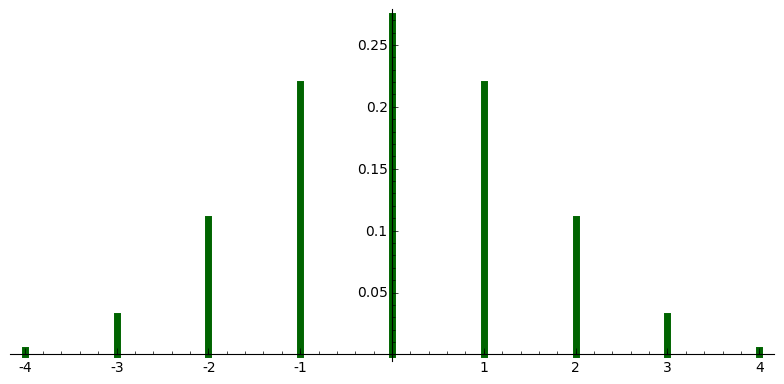
\includegraphics[width = 0.5\textwidth]{v8.png}
\caption{Probability density function of $\cV_8$}
\end{figure}


\begin{Definition}[Modified error distribtuion]
Let $K = \bQ(\zeta_m)$ with degree $n$ ring of integers $R$. Let $q$ be a prime and let $k \geq 2$ be an even integer. Then a sample from the distribtuion $PD_{m,q,k}$ is
\[
    e = \sum_{i=0}^{n-1} e_i \zeta_m^{i} \pmod{qR},
\]
where the $e_i$ are sampled independently from $\cV_k$.
\end{Definition}

{\bf Assumption} Keeping the above notations, $\cR = (K, q, \sigma, s)$ be an RLWE instance. We assume that the distribtutions $PD_{m,q,[\sqrt{2\pi}\sigma]}$ are $D_\cR$ are ``close modulo $\fq$'', in the sense that the two distributions $PD_{m,q,[\sqrt{2\pi}\sigma]} \pmod{\fq}$ and
$D_\cR \pmod{\fq}$ are indistinguishable.

We will analyze the distance between $PD_{m,q,[\sqrt{2\pi}\sigma]} \pmod{\fq}$ and the uniform distribution over $R/\fq$.

\subsection{Fourier analysis}
We recall the definition and key properties of Fourier transform over finite fields.
Suppose $f$ is a real-valued function on $\bF_q$. The {\it Fourier transform} of $f$ is defined as
\[
    \hat{f}(s) = \sum_{a \in \bF_q} f(a) \bar{\chi_s}(a),
\]
where $$\chi_s(a) := e^{2 \pi i as/q}$$

We have the inversion formula:
\[
    f(a) = \frac{1}{q} \sum_{s \in \bF_q} \hat{f}(s)\chi_s(a).
\]

Let ${\bf 1}$ denote the constant function $f \equiv 1$, and let $\delta$ denote the characteristic function of the
one-point set $\{0\} \subseteq \bF_q$.

\begin{Prop} \hfill \\
\begin{enumerate}
\item The transform of the $\delta$ function is $\hat{\delta} = {\bf 1}$.

\item The transform of {\bf 1} is $\hat{{\bf 1}} = q\delta$; if $U$ the uniform distribution over $\bF_q$, then $\hat{U} = \delta$.

\item convolution becomes product.

%\item Plancherel's formula states that
%$||f||_2 = \frac{1}{q} ||\hat{f}||_2$.

%\item $\hat{f(a - \lambda)}(s) =  \bar{\chi_s(\lambda)} f(s)$.
\end{enumerate}
\end{Prop}







\begin{Lemma}
For all even integers $k \geq 2$,
$$\hat{\cV_k}(s)  = \cos \left(\frac{\pi s}{q}\right)^k, (\forall s \in \bF_q).$$
\end{Lemma}

\begin{proof}
Routine calculation.
\end{proof}

Now we consider the error distribution we obtained from mapping RLWE errors to $\bF_q$.

\begin{Definition}
Suppose ${\bf a} = a_1, \cdots ,a_n$ is a vector in $\bF_q^n$. Define the following random variable with
values in $\bF_q$
\[
    e({\bf a}, k, q) := \sum_{i=1}^n a_i e_i \pmod {q}
\]
where the $e_i$ are independent variables with distribution $\cV_k$. Let $E$ denote its probability density function:
$E(b) = \prob(e = b)$ for $b \in \bF_q$.
\end{Definition}

Next, using the fact that the probability of a sum of two varaibles is a convolution, we prove
\begin{Lemma}
\[
    \hat{E_{{\bf a}, k, q}}(s) = \prod_{i=1}^{n} \cos \left(\frac{ a_i \pi s}{q} \right)^k
\]
In particular, $\hat{E}(0) = 1$ for all ${\bf a}$, $k$ and $q$.
\end{Lemma}

\begin{proof}
Routine calculation.
\end{proof}





%\begin{equation*}
%\label{eq:1}
%    ||P - U||_2  = \frac{1}{q}||\hat{P} - \delta||_2.
%\end{equation*}

Next we restrict our attention to cyclotomic fields. Let
$m \geq 1$ be an integer and let $q \equiv 1 \pmod{m}$ be a prime. Then $q$ splits completely in the cyclotomic field $K = \bQ(\zeta_m)$. Let $\alpha \in \bF_q$ be a primitive $n$-th root of unity. Let
\[
    e = e(\alpha) = \sum_{i=0}^{n-1} e_i \alpha^i.
\]
Then $e \gets PD_{m,q,k}$. Let $E$ denote its density function of $e$. Recall that $U$ denotes the density function of the uniform distribution: $U(a) = 1/q$ for all $a \in \bF_q$. Now We can compute $(E - U)(a)$ for any $a \in \bF_q$ using the Fourier inversion formula, using the notations in the beginning of this section,

\begin{align*}
    E(a) - U(a) &= \frac{1}{q} \sum_{s \in \bF_q} (\hat{E}(s) - \hat{U}(s) )\chi_s(a) \\
& = \frac{1}{q} \sum_{s \in \bF_q} (\hat{E}(s) - \delta(s) )\chi_s(a) \\
& = \frac{1}{q} \sum_{s \in \bF_q, s \neq 0} \hat{E}(s) \chi_s(a).
\end{align*}

Since $|\chi_s(a)| \leq 1$ for all $a$ and all $s$, we have

\begin{Prop}
\[
    \boxed{|E(a) -  1/q| \leq \frac{1}{q}  \sum_{y \in \bF_q, y \neq 0}  |\hat{E}(y)|, \, (\forall a \in \bF_q)}
\]
\end{Prop}

Let $\epsilon(m,q,k,\alpha)$ denote the right hand side of the above inequality, i.e.,
\[
    \epsilon(m,q,k, \alpha) = \frac{1}{q}\sum_{y \in \bF_q, y \neq 0} \prod_{i=0}^{n-1} \cos \left(\frac{ \alpha^i \pi y}{q} \right)^k.
\]
We let $\alpha$ run over all primitive n-th root of unities in $\bF_q$ and define
$$\epsilon(m,q,k) := \max_{\alpha: \varphi_m(\alpha) = 0 } \epsilon(m,q,k,\alpha)$$
The punchline of our argument is: the value $\epsilon(m,q,k)$ is usually negligibly small. As a result, the distribution $PD_{m,q,k} \pmod {\fq}$ is computationally indistinguishable from uniform for all $\fq$. The following is a table of data, to demonstrate how small it is.

\FloatBarrier
\begin{table}[H]
\caption{$f = 1$}
\begin{tabular}{c|c|c}
$m$ & $q$ & $[\log_2(\epsilon(m,q, 2))]$ \\
\hline
244 & 1709 & $-230$ \\
101 & 1213 & $-177$ \\
256 & 3329 & $-194$ \\
256 & 14081 & $-208$ \\
55 & 10891  & $-44$ \\
197 & 3547 & $-337$ \\
96 & 4513 & $-35$ \\
160 & 20641 & -61 \\
145 & 19163 & $-176$ \\
101 & 101 & $-4$ \\
13 & 1000039 & $-12$ \\
512 & 7681 & -455  \\
512 & 10753 & -431 \\
512 & 19457 & -414
\end{tabular}
\end{table}

On row $-1$ and $-2$ from the above table, we can see the effect of taking the ramified prime, or taking $q \gg n$.



\begin{remark}
It is possible to generalize this cryptoanalysis to higher degree primes, where we are looking at general finite fields $\bF_{q^f}$. In this situation we should interpret
$\chi_s(a) = e^{2 \pi i Tr(as)/q}$. Separability tells us this is an isomorphism between $\bF_q$ and its dual, and we can define the Fourier transform this way. So everything goes through? We just want to add a trace to everything, i.e.,

\[
    \hat{E_{{\bf a}, k, q}}(s) = \prod_{i=1}^{n} \cos \left(\frac{ \pi Tr(a_i s) }{q} \right)^k
\]
Note this is well-defined when $k$ is even, which we always assume.
\end{remark}


We have a table for degree 2 primes.
\FloatBarrier
\begin{table}[H]
\caption{$f = 2$}
\begin{tabular}{c|c|c}
$m$ & $q$ & $-[\log_2(\epsilon(m,q,2))]$ \\
\hline
53 & 211 & 61 \\
55 & 109 & 48 \\
63 & 881 & 33 \\
64 & 127 & 37 \\
64 & 191 & 35 \\
64 & 383 & 31 \\
512 & 257 & 263
\end{tabular}
\end{table}

In terms of statistical distance, ...,

\section{Conclusion and open problems}

\bibliographystyle{amsalpha}
\bibliography{galois-rlwe}

\end{document}
